\documentclass[11pt,a4paper]{article}
\usepackage[T1]{fontenc}
\usepackage[utf8]{inputenc}
\usepackage{lmodern,microtype}
\usepackage[margin=22mm,headheight=15pt]{geometry}
\usepackage{amsmath,amssymb,booktabs,longtable,tabularx,array}
\usepackage{graphicx,xcolor,enumitem,fancyhdr,placeins,xurl,needspace}
\usepackage{tikz}
\usetikzlibrary{positioning,arrows.meta}
\usepackage{hyperref}
\definecolor{ink}{HTML}{183444}
\definecolor{accent}{HTML}{087F8C}
\definecolor{warm}{HTML}{C76435}
\definecolor{soft}{HTML}{EDF5F6}
\hypersetup{colorlinks=true,linkcolor=accent,urlcolor=accent,citecolor=accent,
 pdftitle={Visual Emotion Trajectories: Hypotheses, Models, and 264 Experiments},
 pdfauthor={Video2Reaction research project}}
\pagestyle{fancy}\fancyhf{}
\fancyhead[L]{\small\textcolor{ink}{Visual emotion trajectories}}
\fancyhead[R]{\small 7 October 2026}
\fancyfoot[C]{\small\thepage}
\renewcommand{\headrulewidth}{0.3pt}
\setlength{\parindent}{0pt}\setlength{\parskip}{5pt}
\setlength{\emergencystretch}{2em}
\setlist{itemsep=3pt,topsep=4pt,leftmargin=*}
\setlist[description]{style=nextline,leftmargin=0pt,labelindent=0pt,labelwidth=0pt}
\renewcommand{\arraystretch}{1.12}
\setcounter{tocdepth}{2}
\newcommand{\KL}{\operatorname{KL}}
\newcommand{\softmax}{\operatorname{softmax}}
\newcommand{\sigmoid}{\operatorname{sigmoid}}
\newcommand{\LN}{\operatorname{LayerNorm}}
\newcommand{\GELU}{\operatorname{GELU}}
\newcommand{\ReLU}{\operatorname{ReLU}}
\newcommand{\tbl}[1]{\input{tables/#1.tex}}
\newcommand{\fig}[3]{\begin{figure}[!htbp]\centering\includegraphics[width=#2\linewidth]{figures/#1.pdf}\caption{#3}\label{fig:#1}\end{figure}\FloatBarrier}
\newcommand{\keypoint}[1]{\par\smallskip\colorbox{soft}{\parbox{0.95\linewidth}{#1}}\par\smallskip}
\raggedbottom

\begin{document}
\hypersetup{pageanchor=false}
\begin{titlepage}
\vspace*{7mm}
{\large\textcolor{accent}{VIDEO2REACTION RESEARCH REPORT}}\par
\vspace{8mm}
{\fontsize{28}{33}\selectfont\bfseries\raggedright\textcolor{ink}{Can emotional moments\newline predict audience reactions?}\par}
\vspace{5mm}
{\Large Visual emotion trajectories, duration,\newline moment selection, and rare emotions}\par
\vspace{7mm}
{\large Hypotheses, model details, 264 completed runs,\newline and comparison with the published benchmark}\par
\vspace{9mm}
\begin{tabularx}{\linewidth}{@{}XX@{}}
\textbf{88 conditions} & \textbf{3 training seeds per condition}\\
16 primary + 72 additional & Seeds 42, 43, and 44\\[5pt]
\textbf{264/264 runs completed} & \textbf{Metrics independently checked}\\
Finished by 01:03 Amsterdam, 7 October & Recomputed from saved predictions\\
\end{tabularx}
\vspace{9mm}
\keypoint{\textbf{Main finding.} A simple model that averages visual features is the strongest configuration by validation score. Its mean test Kullback--Leibler divergence, a measure of probability-distribution error, is \textbf{0.580511}; lower is better. The best tested model that decodes emotions through fixed valence--arousal--dominance coordinates scores \textbf{0.835698}. The proposed trajectory and peak mechanisms have therefore not improved this visual baseline.}
\vspace{4mm}
The visual baseline's score is numerically below the paper's 0.588 reference, but its reaction-ranking and classification scores are lower. We do not claim an overall win over the paper. The wide baseline's small gain over ordinary mean pooling is also statistically inconclusive.

This report explains the full prediction path, the controls that test each hypothesis, the numerical results, and the limits of the conclusions. Complete condition scores and all 264 job IDs are included in the appendices.
\vfill
\textbf{Report date:} 7 October 2026\par
\textbf{Execution:} Snellius; locked uv environment; official dataset splits\par
\textbf{Research branch:} \path{research/video2reaction-experiments}\par
\textbf{Scope:} Pure visual inputs with fixed numerical emotion coordinates; no text proxy\par
\end{titlepage}

\pagenumbering{roman}
\hypersetup{pageanchor=true}
\tableofcontents
\clearpage
\pagenumbering{arabic}

\section{The question we are testing}
\subsection{From a video to a distribution of reactions}
The task is to predict how an audience reacts to a video. The answer is a probability distribution over 21 reactions, rather than a single emotion label. A clip might induce amusement in some viewers, admiration in others, and disapproval in another group. These reactions need not match the facial expressions or mood shown on screen.

Let $y_c$ be the target probability of reaction $c$, and let $P_c$ be the model's prediction. Both are nonnegative and sum to one across the 21 categories. The targets are the dataset's existing audience-reaction distributions. Individual comments are not inputs to the models in this report.

The central proposal is that most reactions concern a few useful moments. A video's emotional state may move through a three-dimensional space: \textbf{valence} describes pleasantness, \textbf{arousal} describes activation or intensity, and \textbf{dominance} describes control or power. We use the abbreviation \textbf{VAD} for these three coordinates after introducing them here.

Under the proposal, a scene near one emotion's coordinates should contribute to that emotion. A longer scene should contribute more evidence if its relevance and proximity are otherwise equal. A brief but highly relevant event might outweigh a longer, less relevant scene. The experiments ask whether learning this combination helps predict the observed reaction distribution.

\subsection{Five hypotheses and the comparisons they require}
\begin{description}
\item[H1: Useful moments.] Learning which scenes matter should improve on duration-weighted averaging. We compare learned soft relevance with duration-only aggregation using the same visual contextual model and local decoder.
\item[H2: Sparse selection.] Allowing some scenes to contribute exactly zero should improve on giving every scene a positive weight. We compare sparse and soft relevance with matched architecture and optimization.
\item[H3: Peak evidence.] A single emotional peak, or a separate closest moment for each emotion, may explain reactions better than accumulated evidence. We compare these peak rules with duration, relevance, and power pooling.
\item[H4: Meaningful VAD geometry.] Fixed human-rated emotion coordinates should help beyond simply compressing a prediction into three dimensions. We compare sourced coordinates with permuted label assignments, and with an unrestricted 21-output local classifier.
\item[H5: Rare reactions.] Increasing the training frequency of clips with rare reaction mass may improve their predictions. An importance-corrected control distinguishes a change in sampling from a change in the expected loss being optimized.
\end{description}

\textbf{What would count as support?} A lower validation-selected test error against the appropriate matched control, with consistent seed behavior and uncertainty that supports the difference. Beating an unrelated baseline alone would not establish that VAD semantics or sparse moment selection caused the gain.

\subsection{What ``pure visual'' means here}
Every learned input is derived from an RGB scene keyframe and its timestamp. The backbone is DINOv2, a visual model trained by self-supervision \cite{dinov2}. No descriptions, captions, audio features, text embeddings, language-model teacher, or comment text enter the prediction path. The existing soft reaction labels are training targets.

The NRC VAD lexicon provides only a fixed numerical coordinate for each output label \cite{nrc}. This is a label prior, not a textual representation of the video. Earlier project models used SigLIP, whose pretraining aligns images and language; their results are discussed separately in Section~\ref{sec:prior}.

\section{Dataset and the information actually observed}
\subsection{Splits, keyframes, and targets}
We preserve the official Video2Reaction split and the fixed class order. Dataset metadata is pinned to revision \path{578d1423f89f1a7b52471b01e78770e08f0a226c} \cite{dataset}. The original data was inspected on Snellius before the new model code was written.

\begin{table}[htbp]\centering
\caption{Observed data inventory. Every listed scene has one indexed keyframe.}
\begin{tabular}{lrrr}\toprule
Split & Clips & Keyframes & Mean keyframes per clip\\\midrule
Training & 7,243 & 317,950 & 43.898\\
Validation & 1,035 & 45,964 & 44.410\\
Test & 2,070 & 91,312 & 44.112\\\midrule
Total & 10,348 & 455,226 & 43.992\\\bottomrule
\end{tabular}\end{table}

All indexed paths exist, and complete feature extraction decoded all 455,226 images. Clips have between 15 and 176 keyframes. A scene index records its start and end times. All audited intervals have positive duration, with no gaps or overlaps. Scene durations range from approximately 0.04 seconds to 138.08 seconds in training.

For each clip, the model observes one static image per indexed scene. It does \emph{not} observe every video frame, optical flow, or motion inside a scene. Its emotional trajectory is therefore a \textbf{piecewise-constant estimate}: one estimated emotional state for each observed interval. A long interval does not establish that the emotion stayed constant throughout that interval.

\subsection{Imbalance and the meaning of a rare reaction}
Rarity is defined from the average \emph{soft probability mass} in training. This differs from counting how often a reaction is the single most common label. Admiration, disapproval, and amusement together account for about 68.59\% of training probability mass. The largest-to-smallest mean-mass ratio is 174.17.

The six lowest-mass training labels are embarrassment, annoyance, nervousness, realization, relief, and caring. They jointly carry 0.018256 of test probability mass. None has target Top-1 support under the official test metric. Consequently, their all-class Top-1 F1 is zero for every model and is not an informative measure of successful rare-emotion recognition here. We instead inspect their probability errors and total predicted mass, while retaining the official metrics.

Appendix~\ref{app:classes} lists all classes in the exact prediction order, together with their training mass and dominant-label counts.

\subsection{Leakage and generalization limits}
There are no duplicate clip IDs across splits. However, \textbf{1,986 of 2,070 test clips (95.94\%) share a movie with training}. Only 84 test clips come from unseen movies. The test set contains 1,183 distinct movie IDs. Movie identity is not a model input, but visual appearance can still reveal movie-specific information.

The official split supports comparison on held-out clips; it does not establish generalization to wholly new movies. Grouping uncertainty estimates by movie helps account for dependence among test clips, but it does not remove training/test movie overlap. Content-level near-duplicate video detection was not performed.

\section{The model, step by step}\label{sec:model}
\subsection{Overview and tensor sizes}
Consider a batch of $B$ videos, padded to $T$ scenes each. A mask marks real scenes so padding contributes no probability mass. For each real scene $i$, we have an image, a start time $s_i$, an end time $e_i$, and duration $\Delta t_i=e_i-s_i$.

The prediction path has two learned branches after visual contextualization: an emotional-state branch and a relevance branch. They are trained together through the final video-level reaction loss. There is no separate ground-truth highlight loss and no supervised VAD regression target in these 264 experiments.

\begin{figure}[htbp]\centering
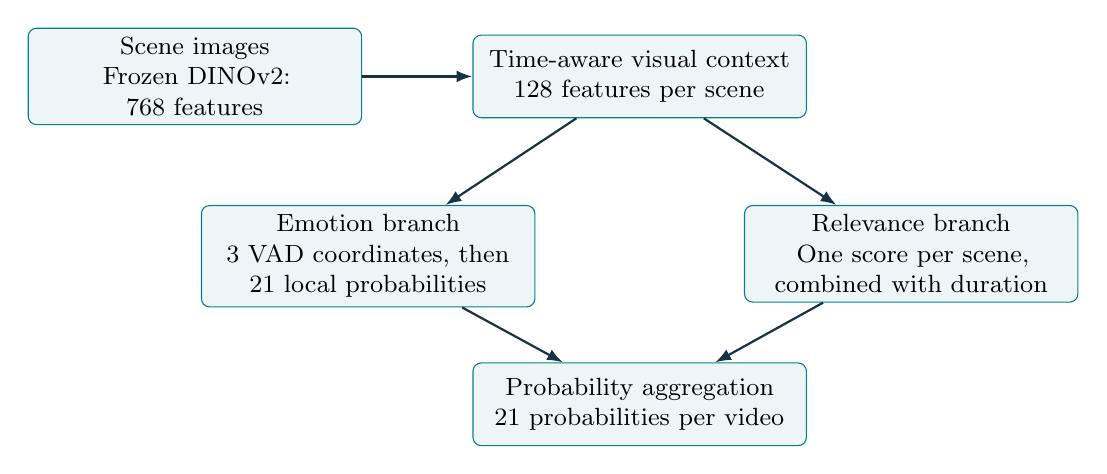
\begin{tikzpicture}[box/.style={draw=accent,rounded corners=3pt,fill=soft,text width=4.0cm,minimum height=1.05cm,align=center,font=\small},arr/.style={-{Latex[length=2mm]},thick,draw=ink},node distance=8mm]
\node[box] (image) {Scene images\\Frozen DINOv2: 768 features};
\node[box,right=14mm of image] (context) {Time-aware visual context\\128 features per scene};
\node[box,below left=11mm and -8mm of context] (emotion) {Emotion branch\\3 VAD coordinates, then\\21 local probabilities};
\node[box,below right=11mm and -8mm of context] (relevance) {Relevance branch\\One score per scene,\\combined with duration};
\node[box,below=31mm of context] (mixture) {Probability aggregation\\21 probabilities per video};
\draw[arr] (image)--(context);
\draw[arr] (context)--(emotion);\draw[arr] (context)--(relevance);
\draw[arr] (emotion)--(mixture);\draw[arr] (relevance)--(mixture);
\end{tikzpicture}
\caption{The VAD trajectory path. The relevance branch is used only in relevance-based variants. The unrestricted controls replace the three-coordinate emotion head with 21 free logits.}
\end{figure}\FloatBarrier

\begin{table}[htbp]\centering
\caption{Main tensor dimensions in the default trajectory model.}
\begin{tabularx}{\linewidth}{p{4.0cm}p{3.5cm}X}\toprule
Quantity & Shape & Meaning\\\midrule
Visual features & $B\times T\times768$ & Frozen image representation\\
Timing packet & $B\times T\times3$ & Duration, start, end in seconds\\
Contextual features & $B\times T\times128$ & Scene representation with video context\\
VAD estimates & $B\times T\times3$ & Learned coordinates bounded to $[-1,1]$\\
Local distributions & $B\times T\times21$ & Reaction probabilities for each scene\\
Temporal weights & $B\times T$ & Scene contributions summing to one\\
Video distribution & $B\times21$ & Final prediction\\\bottomrule
\end{tabularx}\end{table}

\subsection{Step 1: encode each image with frozen DINOv2}
The backbone is \path{facebook/dinov2-base}, pinned to revision \path{f9e44c814b77203eaa57a6bdbbd535f21ede1415}. Its image Transformer has 12 layers, 12 attention heads, 768-dimensional hidden states, and $14\times14$ image patches. An attention head lets the model compare one image region with other regions; multiple heads learn different comparisons.

The actual cached processor resizes the shorter image edge to 256 pixels with bicubic interpolation, center-crops $224\times224$ pixels, rescales by $1/255$, and normalizes RGB channels by means $(0.485,0.456,0.406)$ and standard deviations $(0.229,0.224,0.225)$. The model configuration's nominal image size is 518; this is not the crop used in these runs. The processor's 224-pixel crop is the operative input size.

We take the final hidden state of the \textbf{classification token}, commonly called the \textbf{CLS token}. Here it serves as a 768-number summary of the image; it is not a pretrained classifier for our 21 reactions. The backbone stays in evaluation mode and is not updated during reaction training. Extraction uses reduced-precision bfloat16 computation; cached features are stored as float32.

\subsection{Step 2: project features and add temporal context}
Each frozen feature $f_i\in\mathbb{R}^{768}$ first passes through layer normalization and a learned linear map:
\begin{equation}
u_i=W_{\mathrm{proj}}\LN(f_i)+b_{\mathrm{proj}},\qquad u_i\in\mathbb{R}^{128}.
\end{equation}
Layer normalization rescales the feature dimensions within one scene. It does not average scenes or mix different videos.

The default model adds a sinusoidal encoding of the scene's actual midpoint time, $m_i=(s_i+e_i)/2$. For hidden width $d=128$ and $k=0,\ldots,d/2-1$,
\begin{align}
\omega_k&=\exp\!\left(-\frac{2k\log10000}{d}\right),\\
\mathrm{time}_{i,2k}&=\sin(m_i\omega_k),\qquad
\mathrm{time}_{i,2k+1}=\cos(m_i\omega_k).
\end{align}
Using seconds distinguishes a short scene from a long scene's location in the clip. The timestamp-free controls remove this encoding, while keeping duration weights and visual contextualization.

Two Transformer encoder layers process the sequence $u_i+\mathrm{time}_i$. Each layer uses four attention heads and a feed-forward subnetwork $128\rightarrow512\rightarrow128$, with rectified linear activation (ReLU). Layer normalization is applied before each sublayer, and a residual connection adds each sublayer's output back to its input. Dropout is zero. These are the settings of the newly trained temporal model; the frozen DINOv2 backbone has its own architecture.

The resulting contextual feature is $h_i\in\mathbb{R}^{128}$. A scene can attend to \emph{all} other scenes in the clip. Its emotional estimate is therefore scene-indexed but conditioned on the whole video. This is an offline predictor, not a causal online tracker or a detector that decides when a video should end.

\subsection{Step 3: turn a scene into a point in VAD space}
The emotional-state branch is a feed-forward network:
\begin{equation}
z_i=\tanh\!\left(W_2\GELU(W_1h_i+b_1)+b_2\right),\qquad z_i\in[-1,1]^3.
\end{equation}
The hidden layer has width 128 and the final layer has three outputs. GELU, the Gaussian error linear unit, is a smooth activation function; $\tanh$ bounds each coordinate between $-1$ and $1$.

The 21 label coordinates $v_c\in[-1,1]^3$ come from exact matching entries in NRC VAD v2.1. The file preserves the benchmark's class order and is checksum-verified. These points remain fixed during training. There are no video captions or text-derived video embeddings in this step.

The distance between scene $i$ and emotion $c$ becomes a positive affinity:
\begin{equation}
k_{ic}=\exp\!\left(-\frac{\lVert z_i-v_c\rVert_2^2}{\tau}\right),\qquad
q_{ic}=\frac{k_{ic}}{\sum_{d=1}^{21}k_{id}}.
\label{eq:distance}
\end{equation}
Here $q_i$ is the scene's probability distribution over reactions. The \textbf{temperature} $\tau$ controls how sharply distances are converted into probabilities. Small values emphasize the closest labels; larger values give a flatter distribution.

One temperature is learned for the whole model:
\begin{equation}
\tau=0.05+1.95\sigmoid(\theta).
\end{equation}
The primary initialization is $0.25$. The overnight sweep initializes it at $0.1$, $0.6$, or $1.2$ instead. It remains trainable in all of those runs, so this is a test of initialization sensitivity, not fixed-bandwidth tuning. The decoder has no free bias for each class and no residual classifier that can bypass the VAD distances.

The sigmoid function maps the learned scalar $\theta$ into $(0,1)$; the scale and offset above keep the temperature between 0.05 and 2.0. A \textbf{logit} is a score before probability normalization. \textbf{Softmax} exponentiates a set of logits and divides by their total, producing probabilities that sum to one. Equation~\ref{eq:distance} is a softmax whose logits are negative squared distances divided by temperature.

\subsection{Step 4: learn which scenes matter}
The relevance scorer is a separate small network:
\begin{equation}
a_i=\frac{w_a^\top\tanh(W_ah_i+b_a)}{T_a}.
\end{equation}
Its dimensions are $128\rightarrow32\rightarrow1$, with no bias in the last layer. The default fixed relevance temperature is $T_a=0.2$. The overnight alternatives are $0.05$, $0.1$, $0.5$, and $1.0$. This temperature is distinct from the learned VAD-distance temperature $\tau$.

The normalized duration of a scene is
\begin{equation}
\mu_i=\frac{\Delta t_i}{\sum_j\Delta t_j}.
\end{equation}
Soft relevance gives each real scene a positive contribution:
\begin{equation}
w_i=\frac{\mu_i\exp(a_i)}{\sum_j\mu_j\exp(a_j)}.
\end{equation}
This is a duration-weighted version of learned attention, related to weakly supervised multiple-instance learning \cite{mil}. A long scene and a high relevance score both increase its contribution.

Sparse relevance can set contributions exactly to zero. It finds a threshold $b$ satisfying
\begin{equation}
\sum_i\mu_i[a_i-b]_+=1,\qquad
w_i=\mu_i[a_i-b]_+,\qquad [x]_+=\max(x,0).
\label{eq:sparse}
\end{equation}
This is our duration-weighted adaptation of sparsemax \cite{sparsemax}. Relevance is treated as a \emph{density over time}; $w_i$ is the probability mass assigned to the entire scene. For fixed scene predictions and relevance, splitting one constant scene into two identical pieces with durations that sum to the original leaves its total contribution unchanged. This property holds at the aggregation stage; it does not assert that a Transformer is invariant to duplicating its input tokens.

\subsection{Step 5: aggregate momentary probabilities}
The main prediction is the mixture
\begin{equation}
P_c=\sum_i w_iq_{ic}.
\label{eq:mixture}
\end{equation}
Because both $w$ and each $q_i$ are normalized, $P$ already sums to one. Different scenes can support different emotions. Averaging the \emph{probabilities} avoids cancelling opposite emotional positions by averaging their coordinates first.

For a simple two-reaction illustration, suppose a six-second scene predicts $(0.9,0.1)$ for joy and fear, while a three-second scene predicts $(0.4,0.6)$. Equal relevance gives
\[
P=\tfrac69(0.9,0.1)+\tfrac39(0.4,0.6)=(0.7333,0.2667).
\]
A higher relevance score for the second scene could reverse the duration advantage. This is a mathematical illustration, not a fitted dataset example.

The actual code computes these expressions in log space using log-sum-exp for numerical stability. Padded positions receive zero weight. The exported per-emotion contributions sum back to the saved video distribution.

\subsection{Alternative aggregation rules}
\begin{description}
\item[Duration only.] Set $w_i=\mu_i$ in Equation~\ref{eq:mixture}. The local decoder and contextual model are still trained.
\item[One global peak.] Choose the scene with the closest approach to any emotion:
\[
i^*=\arg\min_i\min_c\lVert z_i-v_c\rVert^2,\qquad P=q_{i^*}.
\]
Equal minima use the earliest scene. This hard choice sends prediction gradients through the chosen scene; it is not independently supervised highlight detection.
\item[One peak for each emotion.] Compute $r_c=\max_i k_{ic}$, then $P_c=r_c/\sum_d r_d$. Each emotion may choose a different scene. The maximum is over raw proximity, not local normalized probability, and relative dwell time is discarded.
\item[Raw proximity with sparse relevance.] Compute $r_c=\sum_iw_ik_{ic}$, then normalize $r$ across reactions. This differs from averaging $q_i$: a scene's total affinity $\sum_c k_{ic}$ affects its influence. Dense regions of the prototype space may therefore be favored.
\item[Power pooling.] For a shared learned exponent $r\in(0,8)$, initialized at one,
\[
s_c=\frac{\sum_i\mu_iq_{ic}^{r+1}}{\sum_i\mu_iq_{ic}^{r}},\qquad P_c=\frac{s_c}{\sum_ds_d}.
\]
At $r=0$ this becomes duration averaging; larger values emphasize high-confidence moments. Duration weighting and categorical normalization are our adaptations of power pooling \cite{power}. This is a peak-sensitive comparison, not an exact model of time spent near an emotion.
\end{description}

\subsection{The two essential visual controls}
\textbf{Unrestricted local decoder.} Keep the same projection, contextual Transformer, hidden layer, relevance scorer, and aggregation. Replace the three-output VAD head with 21 learned logits followed by a softmax. This removes fixed emotion geometry while retaining a local probability mixture. The default VAD model declares 517,572 trainable parameters; the free decoder declares 519,893. The small output-head difference is part of the comparison.

\textbf{Visual mean-pooling baseline.} Normalize and project each DINO feature, average the projected features equally across scenes, and apply a feed-forward classifier:
\begin{equation}
\bar u=\frac{1}{T}\sum_{i=1}^{T}\bigl(W\LN(f_i)+b\bigr),\qquad
P=\softmax\!\left(W_o\GELU(W_h\bar u+b_h)+b_o\right).
\end{equation}
This baseline uses no temporal Transformer, timestamp encoding, learned scene selection, or VAD distance decoder. Width 128 gives 119,189 trainable parameters; width 256 gives 269,589. It is a useful simple visual reference, but not a capacity-matched isolation test of attention pooling.

Parameter counts include modules declared trainable even when a variant does not use them in its prediction. For example, duration-only and peak rules do not train the relevance scorer through the output loss.

\section{Training and the experiment matrix}
\subsection{Loss, optimizer, and checkpoint selection}
The training objective is forward \textbf{Kullback--Leibler divergence}, abbreviated \textbf{KL} after this definition. It measures disagreement between the target distribution $y$ and predicted distribution $P$:
\begin{equation}
L=\frac{1}{N}\sum_{n=1}^{N}\sum_{c=1}^{21}y_{nc}\log\frac{y_{nc}}{P_{nc}}.
\end{equation}
Assigning very little probability to a reaction that has substantial target mass is costly. A lower KL is better; zero means matching the target distribution exactly. The evaluation implementation retains the benchmark's numerical stabilization, described in Section~\ref{sec:metrics}.

All runs use AdamW, an adaptive optimizer with weight decay, with learning rate $0.0003$, weight decay $0.0001$, batch size 64, and gradient norm clipped at one. The schedule is constant. Training lasts at most 50 epochs; an epoch processes one training set's worth of examples. Early stopping uses natural-distribution validation KL, patience eight epochs, and an improvement threshold of $0.0001$. The selected checkpoint is the saved checkpoint with the best accepted validation KL, not the last epoch or the best test score.

Seeds 42, 43, and 44 control initialization and sampling. They are all retained. Shared components are initialized consistently within matched configurations, but each aggregation rule trains its own decoder end to end. Thus comparisons test complete learning rules, not different pooling formulas applied to identical fitted local predictions.

\subsection{Rare-reaction sampling and its control}
Let $\pi_c=N^{-1}\sum_n y_{nc}$ be class $c$'s average training mass. For a training clip, calculate
\begin{equation}
r_n=\sum_c y_{nc}\max(\pi_c,10^{-12})^{-\alpha},\quad
\widetilde r_n=\min\!\left(\frac{r_n}{N^{-1}\sum_jr_j},3\right),\quad
p_n=\frac{\widetilde r_n}{\sum_j\widetilde r_j}.
\end{equation}
Each epoch draws $N$ clips with replacement using probabilities $p_n$. The primary exponent is $\alpha=0.5$; the extension also tests $0.25$ and $1.0$. Targets are unchanged. Larger $\alpha$ emphasizes rare-reaction mass more strongly, subject to the cap.

Ordinary training on these draws changes the expected objective. The \textbf{importance-corrected} version instead weights each sampled clip's loss by $1/(Np_n)$. Since
\[
\sum_np_n\frac{L_n}{Np_n}=\frac{1}{N}\sum_nL_n,
\]
its expected loss is the original natural-distribution loss. This control helps separate effects of resampling from effects of optimizing a different target population. All prevalence estimates use training labels only.

\subsection{Primary batch: 16 conditions, 48 runs}
The primary batch includes duration, single peak, per-emotion peak, soft relevance, sparse relevance, power pooling, raw proximity, permuted prototypes, rare sampling with corrected controls, unrestricted local classifiers, a timestamp-free control, and the DINO mean-pooling baseline. Table~\ref{tab:primary} reports all primary scores. Conditions P01--P16 in the appendices preserve their exact configuration names.

\subsection{Overnight extension: 72 conditions, 216 runs}
The extension changes one declared component at a time relative to an existing base condition:
\begin{table}[htbp]\centering\small
\caption{Additional conditions in the overnight batch. Every condition uses three seeds.}
\begin{tabularx}{\linewidth}{p{5.2cm}rX}\toprule
Change & Conditions & Values or matched scope\\\midrule
VAD-temperature initialization & 21 & Three alternatives across seven pooling rules\\
Relevance temperature & 12 & Four alternatives for soft, sparse, raw-proximity pooling\\
Remove timestamp encoding & 8 & Additional VAD and free-decoder controls\\
Increase hidden width to 256 & 6 & VAD/free predictors and mean-pooling reference\\
Rare-sampling strength & 8 & Two exponents; duration/sparse; corrected/uncorrected\\
Rare sampling with free decoders & 4 & Soft/sparse; corrected/uncorrected\\
Free duration and power decoders & 2 & Same aggregation without fixed VAD geometry\\
Additional semantic permutations & 6 & Two permutations for duration/soft/sparse\\
Reduce context to one layer & 5 & Matched VAD/free comparisons\\\midrule
Total & 72 & 216 runs\\\bottomrule
\end{tabularx}\end{table}\FloatBarrier

The additional permutation seeds are 314159 and 161803; the original sparse permutation uses 271828. The sourced coordinates themselves are never changed. A permutation changes which emotion label is assigned to each coordinate.

This is an \textbf{exploratory expansion}. Some primary test scores had been inspected before the overnight matrix was designed. Validation remains the selection criterion, but the full expanded study should not be presented as an untouched confirmatory test of a method fixed in advance.

\section{Evaluation and verification}\label{sec:metrics}
\subsection{Distribution, ranking, and classification scores}
The benchmark measures different aspects of prediction. One method can improve distribution error while losing on identifying the most common reaction. We preserve the upstream metric definitions and class order.

\begin{description}
\item[KL divergence.] The primary selection metric. The reported implementation averages $\sum_c y_c\log(y_c/(P_c+10^{-10})+10^{-10})$ across clips. Lower is better.
\item[Chebyshev distance.] The largest absolute class-probability error in a clip, averaged across clips. Lower is better.
\item[Clark distance.] The square root of summed relative squared class errors, using the reference $10^{-8}$ denominator stabilization. Lower is better.
\item[Cumulative absolute difference (CAD).] Sum of absolute differences between cumulative target and prediction probabilities in the fixed label order, after row normalization. Lower is better. Reordering labels would change this metric.
\item[Cosine similarity and intersection.] Cosine compares the angle between probability vectors; intersection sums the minimum target/predicted mass for each class. Higher is better.
\item[Mean reciprocal rank (MRR).] Rank the model's predictions and take the reciprocal rank of the target's most probable class, then average over clips. Higher is better.
\item[Target-dominant probability error (TPE).] Absolute probability error at the target's most probable class. Lower is better.
\item[Top-$k$ F1.] Mark the $k$ highest-probability classes in each target and prediction. For each class, combine precision and recall into F1, then weight its F1 by its target support. The normalizer is the total support, $Nk$. Higher is better. We report $k=1,2,3$ as F1@1, F1@2, and F1@3.
\end{description}

Ties matter. Top-$k$ uses NumPy's argsort convention, even if zero-probability labels must enter a Top-$k$ set. MRR uses a target argmax, which can resolve ties differently. The official scores were recomputed with the cluster's NumPy 2.2.6; the report builder on the Mac only formats the verified numbers.

Rare-reaction diagnostics additionally include mean absolute probability error (MAE), group probability mass, and the Brier score, the mean sum of squared probability errors. A probability error can be meaningful even when a class has no dominant-label examples.

\subsection{Uncertainty across clips and across training seeds}
Each reported condition score is the arithmetic mean of three separately trained models' scores. It is \emph{not} a score from averaging their prediction vectors into an ensemble. The sample standard deviation describes variation across those three seeds.

For a paired comparison, we calculate each test clip's loss difference and average that difference across the three trained seeds. We then resample the 1,183 test movies with replacement 10,000 times, retaining all clips from each sampled movie. Dividing the summed loss difference by the sampled clip count preserves the benchmark's clip-weighted mean. The 2.5th and 97.5th percentiles form the reported 95\% interval.

A negative difference favors the first model. An interval that includes zero does not establish a consistent advantage under this resampling scheme. These intervals are conditional on the trained models: they do not resample the training process, remove movie overlap, or correct for testing many exploratory conditions. The random seed for this analysis is 20261007.

\subsection{What was checked independently}
Audit job \textbf{27711358} completed successfully in 3 minutes 44 seconds. It recomputed all validation and test metrics for the 264 new runs, plus five earlier reference runs, from saved predictions to absolute tolerance $10^{-10}$. It checked matching sample IDs, movie IDs, targets, class order, frame counts, 1,035/2,070 unique validation/test clips, selected-epoch scores, checkpoint files, and exact-reload flags. Per-class probability MAE also recomputed for every new run.

Training-time exports assert that per-scene contributions reconstruct predictions. This audit checked the recorded assertions but did not independently reload and recompute every large trajectory tensor. No ground-truth scene-level emotion or viewer-comment alignment was available for a temporal localization audit.

\section{Results}
\subsection{The strongest tested visual predictor}
The lowest mean validation KL belongs to mean pooling with hidden width 256: validation 0.585566 and test 0.580511. Ordinary width-128 mean pooling is almost identical at 0.580898 test KL. The difference is $-0.000386$, with 95\% interval $[-0.002199,+0.001402]$. The wide model therefore gives a small numerical gain, not a demonstrated robust improvement.

\tbl{selected}

The best VAD condition by validation score is soft relevance initialized with distance temperature 0.1. Its test KL is 0.835698, versus 0.580898 for standard mean pooling. The paired difference is $+0.254801$, with interval $[+0.244745,+0.265172]$. The gap is much larger than the small differences among unrestricted visual predictors.

\fig{overview}{1}{Selected test results. Bars show means across three seeds; error bars show seed standard deviations, not confidence intervals. The dashed line is standard DINO mean pooling. Teal denotes unrestricted classifiers and orange denotes fixed-VAD decoders.}

\subsection{All primary hypotheses under the default settings}
\tbl{primary}

\textbf{Useful moments and sparsity.} With unrestricted local logits, soft relevance scores 0.583717 and sparse relevance 0.583976. Their paired difference is small and its interval includes zero. Soft relevance versus a free duration mixture is also inconclusive. These controls do not establish that learned sparse selection improves the probability-distribution prediction.

\textbf{Peak evidence.} The default single-peak VAD rule is especially weak at 1.800579. Per-emotion peak pooling scores 1.094466. Selecting a nearby prototype is not enough to identify a useful scene for audience prediction under this model and training budget.

\textbf{Meaningful coordinate assignments.} Sourced sparse VAD scores 1.069716, while the original permuted-label control scores 0.927439. The permuted-minus-sourced difference is $-0.142277$, with interval $[-0.156808,-0.128307]$. This does not support the claim that the original semantic coordinate assignment is providing the desired advantage in this implementation.

\subsection{What the overnight sweep changed}
\fig{temperature}{0.92}{Mean test KL for four VAD-temperature initializations. The temperature is learned after initialization. This figure shows the whole declared grid; model selection uses validation scores, not the lowest test cell.}

Lowering the initial temperature from 0.25 to 0.1 substantially helps soft VAD: test KL falls from 1.058816 to 0.835698. It remains far behind unrestricted visual prediction. This sensitivity is evidence about optimization and calibration, not proof that the best initialization is universally correct.

The extended free duration and power models score 0.583868 and 0.583673. A one-layer free sparse model scores 0.582423, but its comparison with two-layer free sparse includes zero. Increasing model capacity, changing timestamps, or adding rare sampling does not produce a clearly better validation-selected model than visual mean pooling. Appendix~\ref{app:full} retains every condition, including unfavorable outcomes.

\subsection{Paired uncertainty}
\tbl{paired}
\fig{paired}{1}{Paired movie-bootstrap intervals for seed-averaged losses. The two panels use different horizontal scales. Intervals crossing zero are inconclusive; they should not be turned into claims of superiority.}

\subsection{Rare emotions: what improved and what did not}
\tbl{rare}
\fig{rare}{1}{Probability diagnostics for the six training-defined rare classes. Lower error is better. The dashed line marks their actual combined probability mass in the test targets.}

Rare sampling increases the exposure of rare-reaction clips during training, but that is not itself evidence of a better predictor. For the free sparse model, test KL worsens from 0.583976 to 0.590981. The difference, $+0.007005$, has interval $[+0.003106,+0.010854]$. Rare-class MAE changes from 0.005599 to 0.005619, offering no improvement in that comparison.

For VAD duration, ordinary rare sampling changes KL only from 0.936387 to 0.935977; its interval includes zero. VAD models also assign substantially more mass to the rare group than its true mass. The best VAD model predicts about 0.06925 for a group whose target mass is 0.01826. Increasing rare probability without matching its distribution is not a successful rare-emotion boost.

These six labels have no target Top-1 support in the test set. Their zero Top-1 macro F1 cannot distinguish the models. Top-2 and Top-3 diagnostic supports also inherit the official treatment of ties and zero-probability labels. Probability MAE, mass, and calibration are therefore essential to interpreting the rare-class question.

\subsection{How concentrated were the learned contributions?}
\tbl{support}
For scene contribution mass $m_i=\sum_c\mathrm{contribution}_{ic}$, the effective number of scenes is $1/\sum_i m_i^2$. Equal mass on ten scenes gives ten; one scene carrying all mass gives one. This is a concentration summary, not a count of verified highlights.

Sparse VAD uses about 14.09 effective scenes on average, while its default duration counterpart uses about 27.63. The learned support is not simply one brief emotional peak. More importantly, the context encoder can still use all scenes even if a final contribution is zero. Attribution weights and causal necessity are different questions.

\subsection{Training behavior and unfinished optimization questions}
\tbl{training}
\fig{learning_curves}{1}{Validation histories for seed 42, taken directly from saved training records. The two panels use different vertical scales. Curves are descriptive; all three seeds, not just the displayed seed, contribute to reported scores.}

Across the 264 runs, 43 reached the 50-epoch limit and 16 selected epoch 50. Both the default VAD duration and single-peak conditions ran all 50 epochs for every seed. Some poorly performing runs may therefore still be optimization-limited. The negative result applies to this model family and fixed training budget; it is not a demonstration that longer training cannot help.

The strongest unrestricted models selected early checkpoints. Wide mean pooling selected epochs 8, 8, and 7; free soft and free sparse selected 3, 4, and 3. This contrast is useful when deciding whether a follow-up should focus on optimization, representation, or the distance decoder itself.

\clearpage
\section{Comparison with the Video2Reaction paper}\label{sec:paper}
We compare with \emph{Video2Reaction: Mapping Video to Audience Reaction Distribution in the Wild}, arXiv:2607.06875v1 \cite{paper}. The table below keeps each cited paper row's context visible. A numerical comparison is not a matched reproduction: input modalities, visual encoders, training procedures, and compute budgets differ.

SA-BFGS is the paper's specialized algorithm for learning label distributions: it optimizes KL using the Broyden--Fletcher--Goldfarb--Shanno numerical optimizer. LLaVA-Next and Qwen2.5-VL are pretrained vision--language models. Their names identify model families; they do not denote variants of our DINO predictor. The paper averages its classical baselines over five training seeds, whereas our new study uses three \cite{paper}.

\begin{table}[htbp]\centering\small
\caption{Published scores and our validation-selected visual model. Arrows show the better direction. A dash means the cited row does not provide that value.}
\begin{tabularx}{\linewidth}{p{4.1cm}Xrrrr}\toprule
Method & Source / inputs & KL $\downarrow$ & MRR $\uparrow$ & F1@1 $\uparrow$ & F1@3 $\uparrow$\\\midrule
Our wide DINO mean pooling & Three-seed mean; visual & 0.5805 & 0.6935 & 0.4782 & 0.5963\\
SA-BFGS & Paper Table 7; visual + text & 0.588 & 0.709 & 0.515 & --\\
SA-BFGS & Paper Tables 5--6; visual + audio + text & 0.5976 & 0.7163 & 0.5283 & 0.6265\\
LLaVA-Next & Paper Table 7; visual & 4.148 & 0.731 & 0.586 & --\\
LLaVA-Next, fine-tuned & Paper Tables 5--6 & 3.1765 & 0.7833 & 0.6521 & 0.7672\\
Qwen2.5-VL, fine-tuned & Paper Tables 5--6 & 3.4431 & 0.7548 & 0.6577 & 0.7725\\\bottomrule
\end{tabularx}\end{table}

Our mean KL is numerically 1.27\% below the 0.588 reference and 2.86\% below 0.5976. Against the Table 7 SA-BFGS row, our mean reciprocal rank is lower by 0.0155 and Top-1 F1 by 0.0368. We therefore have a favorable KL number, but \textbf{not an overall paper-beating result}. The paper's strong dominant-reaction scores remain above ours. No paired significance claim against the paper is possible from aggregate published values alone.

The improvement over these KL references comes from the simple visual baseline. It is not evidence for the proposed VAD or peak-emotion mechanism. The best VAD condition does not reach those KL references. We retain this distinction because otherwise a favorable baseline score could be incorrectly attributed to the research hypothesis.

\subsection{Relation to earlier project results}\label{sec:prior}
Earlier experiments used a different frozen visual representation and, in some cases, supplied text descriptions. Their role is historical context, not a matched control for the new DINO trajectory study.

\begin{table}[htbp]\centering
\caption{Earlier project results, each from one training seed. These do not share the new three-seed DINO protocol.}
\begin{tabularx}{\linewidth}{p{5.7cm}Xr}\toprule
Model & Representation / inputs & Test KL\\\midrule
SigLIP mean pooling (B1) & Image input; language-aligned pretraining & 0.544414\\
SigLIP shared attention & Image input; language-aligned pretraining & 0.540655\\
Visual + description fusion & Explicit visual and text inputs & 0.509952\\\bottomrule
\end{tabularx}\end{table}

The earlier lower scores show that changing the backbone and input information matters. They cannot be used as pure DINO-model evidence, and the description model does not meet the requested visual-only input constraint. The previous report and its 41-run audit remain available separately \cite{earlier}.

\section{What the evidence means}
\subsection{A likely bottleneck: the constrained distance decoder}
The matched free-output controls provide the strongest clue. Keeping visual context and probability aggregation while removing fixed VAD geometry gives much better predictions. This suggests that the constrained decoder is a major limitation \emph{in this implementation}.

We can see the restriction by expanding the squared distance in Equation~\ref{eq:distance}. Terms common to every class cancel inside the softmax:
\begin{equation}
q_i=\softmax_c\!\left(\frac{2z_i^\top v_c-\lVert v_c\rVert^2}{\tau}\right).
\end{equation}
Thus the 21 local logits are controlled by a three-dimensional point, a shared temperature, and fixed prototype norms. There is no independently learned class prior. Emotion words that are close in VAD space must have related local probabilities even if their audience-reaction frequencies differ greatly.

This does not prove that the final video distribution has only three degrees of freedom: mixtures of many scene distributions can be richer. Nor does it establish an unavoidable mathematical lower bound on achievable error. Optimization sensitivity, the limited visual representation, full-video conditioning, and the 50-epoch ceiling remain possible contributing factors.

\subsection{Does the code actually reflect the hypotheses?}
\begin{enumerate}
\item \textbf{Duration and proximity enter the calculation.} Actual interval seconds weight the local probabilities; a distinct raw-proximity arm tests the order of normalization.
\item \textbf{Peaks are explicitly tested.} There is one global closest scene and a separate closest scene for each emotion. These are model-defined peaks, not independently labeled emotional events.
\item \textbf{Sparse relevance is learnable.} It can set scene contributions to zero, with matched soft controls. The aggregate clip loss provides its only supervision.
\item \textbf{Fixed VAD coordinates are truly fixed.} There is no hidden text-video representation, residual classifier, or class-bias bypass in the VAD arm. Free decoders are labeled controls.
\item \textbf{Rare sampling is isolated.} Natural, reweighted, and importance-corrected comparisons preserve the same soft targets and validation selection.
\item \textbf{Temporal-order perturbation preserves duration.} When scenes are shuffled for diagnostics, each visual feature travels with its original duration and a new contiguous timeline is built. Otherwise an order test would also change which scene receives each duration weight.
\end{enumerate}

\subsection{What a negative result does and does not reject}
The results do not support useful sparse selection, peak dominance, or a semantic VAD advantage under the tested representation and supervision. They do not disprove every model in which comments concern a few emotional moments. The data representation is sparse in time, the local estimates are weakly supervised, and no independent viewer-moment annotations identify the latent trajectory.

Conversely, a future improvement in clip KL would not by itself prove that attention found the scenes that viewers commented on. Many latent explanations can produce the same clip distribution. A causal or alignment claim would need independent temporal evidence or carefully controlled interventions.

\subsection{Next experiments that would be informative}
These are recommendations, not runs already conducted:
\begin{enumerate}
\item \textbf{Separate decoder calibration from geometric structure.} Compare a train-label prior or a calibrated residual head with fixed VAD, free logits, and permuted-coordinate controls. Such a change relaxes the strict distance-only hypothesis and must be labeled accordingly.
\item \textbf{Check optimization before rejecting the representation.} Extend training only for configurations still improving at the cap, with a matched budget control and validation-only decisions. First test whether they can fit a larger, balanced training subset.
\item \textbf{Observe time more densely.} Use multiple frames or short visual clips within scenes, then compare fixed-second windows, matched random/uniform windows, and smoothed peaks. The present one-keyframe-per-scene approximation cannot settle within-scene dwell-time claims.
\item \textbf{Use temporal supervision if available.} Evaluate selected intervals against independent emotional-moment or viewer-comment alignment annotations. Add a separate highlight objective only when its target and interpretation are explicit.
\item \textbf{Use a suitable rare-reaction evaluation.} Keep official scores, but predefine supported rare-class probability and calibration measures, and obtain enough dominant rare examples for a meaningful classification assessment.
\end{enumerate}

\section{Execution, provenance, and reproduction}
\subsection{Environment and resource use}
All real-data extraction, training, and metric audits ran on Snellius with \path{uv run --frozen --no-sync}. The environment includes Python 3.11.16, PyTorch 2.8.0 with CUDA 12.8, NumPy 2.2.6, Transformers 4.57.1, and scikit-learn 1.7.2. The Mac was used for source changes, synthetic tests, and formatting saved report data. The full dataset and feature cache were not copied to it.

The DINO cache job \textbf{27682121} completed in 1 hour 5 minutes 5 seconds on an A100 GPU. Predictor jobs used A100 multi-instance GPU slices, called \textbf{MIG slices}, with four CPUs and 24 GiB host memory. The primary batch allowed two concurrent predictors with 45-minute limits; the extension allowed eight with 20-minute limits. Actual predictor runtimes ranged from 62 to 324 seconds, with median 121 seconds. Across 264 jobs, this was 10.55 allocated MIG-slice hours, not 10.55 hours of serial wall time or full-GPU time.

\subsection{Smoke tests and the unattended overnight chain}
The primary smoke used three official training clips, eight chronological keyframes each, and checked every one of 16 model variants. A first attempt at learning rate 0.003 failed the single-peak loss-decrease check. The shared rate was corrected to 0.0003 before full benchmarks. A ten-minute retry then timed out; the same corrected source passed within its original twenty-minute limit as job \textbf{27681517}, in 16 minutes 31 seconds. These fitting scores are infrastructure checks on training examples, not generalization results.

The overnight smoke split 72 additional conditions across four jobs, 18 conditions each. Each used the same three videos and 24 keyframes, with 20 fitting updates, exact reload/resume checks, finite normalized outputs, and contribution reconstruction. Each also passed 185 tests. The full 216-run launcher depended on successful completion of all four and verified exact source identity and complete variant coverage before submission.

\begin{table}[htbp]\centering\small
\caption{Overnight control jobs. Times are Amsterdam time (CEST, UTC+2).}
\begin{tabular}{llll}\toprule
Purpose & Job ID & Start & Finish\\\midrule
Smoke shard 0 & 27684811 & Oct 6, 22:55:55 & 23:04:21\\
Smoke shard 1 & 27684812 & Oct 6, 22:55:55 & 23:03:57\\
Smoke shard 2 & 27684813 & Oct 6, 22:55:59 & 23:04:30\\
Smoke shard 3 & 27684814 & Oct 6, 22:57:01 & 23:05:17\\
216-run launcher & 27684815 & Oct 6, 23:05:26 & 23:16:11\\
Morning snapshot & 27684816 & Oct 7, 06:00:03 & 06:00:32\\\bottomrule
\end{tabular}\end{table}

All 264 predictors finished by October 7 at 01:03:13. The scheduled morning snapshot recorded 265 completed jobs: those predictors plus the feature cache. It ran without a laptop process. The independent metric audit was performed later and should not be confused with the 06:00 scheduler snapshot.

\subsection{Source identities and saved artifacts}
The primary runs use source commit \path{05336113586d3686a5cdc58099f0a0d717a435cc}, frozen as \path{05336113586d-bd1c51a39c84}. The extension uses \path{60d7d05a4bf8a17933e061977d6f9909728a521f}, frozen as \path{60d7d05a4bf8-ff5706bd4523}. The audit script was committed as \path{28e01f5}. Results and model configuration identities are retained separately from later report edits.

Cluster root: \path{/scratch-shared/gmago/video2reaction}. Each predictor's output directory is \path{outputs/experiments/<configuration>_s<seed>_<jobid>/}. It contains the resolved configuration, source and environment records, training history, selected and last checkpoints, and validation/test predictions and metrics. Trajectory runs also save per-scene probabilities, affinities, durations, relevance and class contributions, with frame identities and checksums.

The fixed NRC v2.1 archive hash is \path{8bcd04831ffda149f683f8d3091c76a3aee138ee3aa1924b67b50b9416d37df0}. The generated 21-label coordinate asset hash is \path{fb2ce00a38d37e6e8b41418a09cb374ad96b51bc9c24c32f0a51bb790a351906}. Private coordinate assets are not redistributed in the report bundle. Split and report-input hashes are recorded in the accompanying manifest.

\subsection{How to reproduce the analysis and document}
On the cluster, from the committed code checkout and with its environment configured:
\begin{quote}\small\ttfamily
source configs/clusters/snellius.env\par
uv run --frozen --no-sync python scripts/analyze\_trajectories.py\par
\hspace*{1em}--root /scratch-shared/gmago/video2reaction
\end{quote}
The command is one logical invocation; the line break above is for page layout. It analyzes existing outputs and does not launch new training. Rebuilding the document uses the report-asset generator and LaTeX commands in the source bundle's README. The generated tables read the audited JSON directly, so scores are not manually transcribed across 88 conditions.

\keypoint{\textbf{Conclusion.} This study establishes a reproducible visual-only baseline and a completed, well-controlled negative result for the tested fixed-VAD trajectory family. It provides a favorable numerical KL comparison with the published benchmark, but no overall score dominance and no confirmed gain from sparse highlights or rare-reaction sampling. The evidence points toward decoder calibration and richer temporal observations as useful next questions, while keeping optimization and supervision limits explicit.}

\begin{thebibliography}{9}
\bibitem{paper} T. Nguyen et al. \emph{Video2Reaction: Mapping Video to Audience Reaction Distribution in the Wild}. arXiv:2607.06875v1, 2026. Tables 5--7 and 16--17. \url{https://arxiv.org/html/2607.06875v1}.
\bibitem{dataset} Information Fusion Lab. \emph{Video2Reaction dataset}. Revision \path{578d1423f89f1a7b52471b01e78770e08f0a226c}. \url{https://huggingface.co/datasets/infofusionlab/Video2Reaction}.
\bibitem{dinov2} Meta AI. \emph{DINOv2: self-supervised visual features}. Official implementation and models. \url{https://github.com/facebookresearch/dinov2}. Pinned model: \url{https://huggingface.co/facebook/dinov2-base/tree/f9e44c814b77203eaa57a6bdbbd535f21ede1415}.
\bibitem{nrc} S. M. Mohammad. \emph{NRC VAD Lexicon v2: Norms for Valence, Arousal, and Dominance for over 55k English Terms}. arXiv:2503.23547, 2025. Experiments use lexicon release v2.1. \url{https://arxiv.org/abs/2503.23547}.
\bibitem{mil} M. Ilse, J. M. Tomczak, and M. Welling. \emph{Attention-based Deep Multiple Instance Learning}. ICML, 2018. \url{https://proceedings.mlr.press/v80/ilse18a.html}.
\bibitem{sparsemax} A. F. T. Martins and R. F. Astudillo. \emph{From Softmax to Sparsemax: A Sparse Model of Attention and Multi-Label Classification}. ICML, 2016. \url{https://proceedings.mlr.press/v48/martins16.html}.
\bibitem{power} Y. Liu et al. \emph{Power pooling: An adaptive pooling function for weakly labelled sound event detection}. arXiv:2010.09985, 2020. \url{https://arxiv.org/abs/2010.09985}.
\bibitem{results} Video2Reaction research branch. \emph{Verified trajectory results and complete job records}. \path{research_notes/trajectory_results.json}; audited by job 27711358. \url{https://github.com/gowreesh-mago/video2reaction/blob/research/video2reaction-experiments/research_notes/trajectory_results.json}.
\bibitem{earlier} Video2Reaction research branch. \emph{Earlier 41-run study and audit}. 5 October 2026. \url{https://github.com/gowreesh-mago/video2reaction/blob/research/video2reaction-experiments/research_notes/final_report.md}.
\end{thebibliography}

\appendix
\clearpage
\section{Class order and imbalance}\label{app:classes}
The class order is fixed for predictions and the cumulative-distance metric. ``Rare'' means one of the six lowest training soft-mass classes. Dominant counts below use metadata labels; official Top-1 tie-breaking can differ.
\tbl{classes}

\clearpage
\section{Complete results for all 88 conditions}\label{app:full}
P01--P16 identify the original 16 conditions; N01--N72 identify the additional 72. Names are the actual YAML configuration stems. Every row averages seeds 42/43/44. Rows are ordered by validation KL. Test standard deviations describe those three trained seeds and are not confidence intervals. No unfavorable condition has been omitted.

Naming guide: \path{vad} means a fixed-coordinate distance decoder; \path{free} means unrestricted local logits. \path{tau010}, \path{tau060}, and \path{tau120} mean initial VAD temperatures 0.1, 0.6, and 1.2. \path{gate005}, \path{gate010}, \path{gate050}, and \path{gate100} mean relevance temperatures 0.05, 0.1, 0.5, and 1.0. \path{notime} removes timestamp encoding; \path{wide} uses hidden width 256; \path{shallow} uses one context layer. \path{rare025} and \path{rare100} set rarity exponents 0.25 and 1.0. The suffix \path{ipw} denotes inverse-probability weighting, the importance-corrected loss described above. \path{perm} is followed by the label-permutation seed. A configuration such as \path{on_vad_duration_free} inherits the duration base but replaces its decoder with free logits.
\tbl{all_conditions}

\clearpage
\section{Every test score by seed}
This table exposes seed variation directly. The last model checkpoint is not necessarily the selected checkpoint; every listed score comes from validation-based checkpoint selection.
\tbl{seeds}

\clearpage
\section{Every experiment job ID}
The base configuration plus seed plus job ID gives the full output directory name described in the reproduction section. The smoke, cache, launcher, and audit jobs are separate from these 264 predictor jobs.
\tbl{jobs}

\clearpage
\section{Terms and symbols at a glance}
\begin{longtable}{p{3.7cm}p{11.5cm}}\toprule
Term or symbol & Meaning\\\midrule\endhead
Reaction distribution & Probabilities over all 21 audience reactions for one clip.\\
VAD & Valence, arousal, and dominance: three numerical dimensions used for the emotion-coordinate decoder.\\
Keyframe / scene & One representative static image and its observed time interval.\\
$f_i$ & Frozen 768-dimensional image feature for scene $i$.\\
$h_i$ & Learned contextual visual feature for scene $i$, usually 128-dimensional.\\
$z_i$, $v_c$ & Predicted scene coordinate and fixed coordinate of emotion label $c$.\\
$q_{ic}$, $P_c$ & Scene-level and final video-level reaction probabilities.\\
$\Delta t_i$, $\mu_i$ & Duration in seconds and duration divided by total observed duration.\\
$a_i$, $w_i$ & Learned scene relevance score and final scene contribution weight.\\
$\tau$, $T_a$ & Learned VAD-distance temperature and fixed relevance temperature. They control different normalizations.\\
Softmax & Exponentiate scores and normalize them to sum to one.\\
Sparse relevance & A normalization that allows exactly zero scene contributions.\\
KL & Kullback--Leibler divergence: discrepancy between target and predicted distributions; lower is better.\\
MRR & Mean reciprocal rank of the target-dominant reaction; higher is better.\\
F1@k & Support-weighted class F1 after converting both distributions to Top-$k$ label sets.\\
MAE & Mean absolute error in probabilities.\\
Epoch / seed & One training set's worth of updates / a setting controlling initialization and random sampling.\\
Bootstrap interval & Uncertainty estimated by resampling observed units; here the units are movies.\\
MIG slice & A partition of an NVIDIA GPU allocated to an individual cluster job.\\
uv & The environment manager used to run the locked Python dependencies on Snellius.\\\bottomrule
\end{longtable}

\end{document}
